
% This Guide contains Library recommendations based mainly on APA and IEEE styles, but you must always follow the guidelines of your TFG Tutor and the TFG regulations for your degree.

% THIS TEMPLATE IS BASED ON THE APA STYLE 


%----------
% DOCUMENT SETTINGS
%----------

\documentclass[11pt]{report} % font: 12pt

% margins: 2.5 cm top and bottom; 3 cm left and right
\usepackage[
a4paper,
vmargin=2.5cm,
hmargin=2cm
]{geometry}

% Paragraph Spacing and Line Spacing: Narrow (6 pt / 1.15 spacing) or Moderate (6 pt / 1.5 spacing)
\renewcommand{\baselinestretch}{1}
\parskip=5pt

% Color settings for cover and code listings 
\usepackage[table]{xcolor}
\definecolor{azulUC3M}{RGB}{0,0,102}
\definecolor{gray97}{gray}{.97}
\definecolor{gray75}{gray}{.75}
\definecolor{gray45}{gray}{.45}
\definecolor{darkgreen}{rgb}{0.0, 0.5, 0.0}
\definecolor{lightgreen}{rgb}{0.5, 1.0, 0.5}
\definecolor{darkred}{rgb}{0.7, 0.0, 0.0}
\definecolor{lightred}{rgb}{1.0, 0.5, 0.5}
\definecolor{lightyellow}{rgb}{1.0, 1.0, 0.5}

% PDF/A -- Important for its inclusion in e-Archive. PDF/A is the optimal format for preservation and for the generation of metadata: http://uc3m.libguides.com/ld.php?content_id=31389625. 

% In the template we include the file OUTPUT.XMPDATA. You can download that file and include the metadata that will be incorporated into the PDF file when you compile the memoria.tex file. Then upload it back to your project. 
\usepackage[a-1b]{pdfx}

% LINKS
\usepackage{hyperref}
\hypersetup{colorlinks=true,
	linkcolor=black, % links to parts of the document (e.g. index) in black
	urlcolor=blue,   % links to resources outside the document in blue
    citecolor=blue}  % cites

% MATH EXPRESSIONS
\usepackage{amsmath,amssymb,amsfonts,amsthm}

% Tables
\usepackage{booktabs} % For elegant table formatting
\usepackage{adjustbox} % To adjust table width if necessary
\usepackage{booktabs} 
\usepackage{longtable}



% Character encoding
\usepackage{txfonts} 
\usepackage[T1]{fontenc}
\usepackage[utf8]{inputenc}
\usepackage{listings}
\usepackage{subcaption} % For subfigures


% English settings
\usepackage[english]{babel} 
\usepackage[babel, english=american]{csquotes}
\AtBeginEnvironment{quote}{\small}

% Footer settings
\usepackage{fancyhdr}
\pagestyle{fancy}
\fancyhf{}
\renewcommand{\headrulewidth}{0pt}
\rfoot{\thepage}
\fancypagestyle{plain}{\pagestyle{fancy}}

% DESIGN OF THE TITLES of the parts of the work (chapters and epigraphs or sub-chapters)
\usepackage{titlesec}
\usepackage{titletoc}
\titleformat{\chapter}[block]
{\large\bfseries\filcenter}
{\thechapter.}
{5pt}
{\MakeUppercase}
{}
\titlespacing{\chapter}{0pt}{0pt}{*3}
\titlecontents{chapter}
[0pt]                                               
{}
{\contentsmargin{0pt}\thecontentslabel.\enspace\uppercase}
{\contentsmargin{0pt}\uppercase}                        
{\titlerule*[.7pc]{.}\contentspage}                 

\titleformat{\section}
{\bfseries}
{\thesection.}
{5pt}
{}
\titlecontents{section}
[5pt]                                               
{}
{\contentsmargin{0pt}\thecontentslabel.\enspace}
{\contentsmargin{0pt}}
{\titlerule*[.7pc]{.}\contentspage}

\titleformat{\subsection}
{\normalsize\bfseries}
{\thesubsection.}
{5pt}
{}
\titlecontents{subsection}
[10pt]                                               
{}
{\contentsmargin{0pt}                          
	\thecontentslabel.\enspace}
{\contentsmargin{0pt}}                        
{\titlerule*[.7pc]{.}\contentspage}  


% Tables and figures settings
\usepackage{tcolorbox}
\usepackage{longtable}
\usepackage{multirow} % combine cells 
\usepackage{caption} % customize the title of tables and figures
\usepackage{floatrow} % we use this package and its \ ttabbox and \ ffigbox macros to align the table and figure names according to the defined style.
\usepackage{eurosym}
\usepackage{array} % with this package we can define in the following line a new type of column for tables: custom width and centered content
\newcolumntype{P}[1]{>{\centering\arraybackslash}p{#1}}
\DeclareCaptionFormat{upper}{#1#2\uppercase{#3}\par}
\usepackage{graphicx}
\graphicspath{{imagenes/}} % images fodler

% Table layout for social sciences and humanities
\captionsetup*[table]{
	justification=raggedright,
	labelsep=newline,
	labelfont=small,
	singlelinecheck=false,
	labelfont=bf,
	font=small,
	textfont=it
}

% Figure layout for social sciences and humanities
\captionsetup[figure]{
	%name=Figura,
	singlelinecheck=off,
	labelsep=newline,
	font=small,
	labelfont=bf,
	textfont=it
}
\floatsetup[figure]{
    style=plaintop,
    heightadjust=caption,
    footposition=bottom,
    font=small
}

% Figures and tables footnote layout 
\captionsetup*[floatfoot]{
    footfont={small, up}
}

% FOOTNOTES
\usepackage{chngcntr} % continuous numbering of footnotes
\counterwithout{footnote}{chapter}

% CODE LISTINGS 
% support and styling for listings. More information in  https://es.wikibooks.org/wiki/Manual_de_LaTeX/Listados_de_código/Listados_con_listings
\usepackage{listings}

% Custom listing
% \lstdefinestyle{estilo}{ frame=Ltb,
% 	framerule=0pt,
% 	aboveskip=0.5cm,
% 	framextopmargin=3pt,
% 	framexbottommargin=3pt,
% 	framexleftmargin=0.4cm,
% 	framesep=0pt,
% 	rulesep=.4pt,
% 	backgroundcolor=\color{gray97},
% 	rulesepcolor=\color{black},
% 	%
% 	basicstyle=\ttfamily\footnotesize,
% 	keywordstyle=\bfseries,
% 	stringstyle=\ttfamily,
% 	showstringspaces = false,
% 	commentstyle=\color{gray45},     
% 	%
% 	numbers=left,
% 	numbersep=15pt,
% 	numberstyle=\tiny,
% 	numberfirstline = false,
% 	breaklines=true,
% 	xleftmargin=\parindent
% }

% \captionsetup*[lstlisting]{font=small, labelsep=period}

\usepackage{listings}
\usepackage{xcolor}

% Optional: Define a custom style for R code
\lstdefinestyle{Rstyle}{
    language=R,
    basicstyle=\ttfamily\footnotesize,
    keywordstyle=\color{blue},
    commentstyle=\color{green!50!black},
    stringstyle=\color{red!70!black},
    numbers=left,
    numberstyle=\tiny\color{gray},
    stepnumber=1,
    breaklines=true,
    frame=tb, % adds a top and bottom rule
    tabsize=2
}


% \lstdefinestyle{ElegantR}{
%     language=R,
%     basicstyle=\footnotesize\ttfamily,
%     backgroundcolor=\color{black!5},
%     keywordstyle=\color{RoyalBlue}\bfseries,
%     commentstyle=\color{ForestGreen}\itshape,
%     stringstyle=\color{Purple},
%     showstringspaces=false,
%     breaklines=true,
%     numbers=left,
%     numberstyle=\tiny\color{Gray},
%     numbersep=8pt,
%     frame=single,
%     framesep=5pt,
%     framerule=0.5pt,
%     rulecolor=\color{black!20},
%     emph={ggplot, aes, geom_point, geom_line, mutate, arrange, filter, select},
%     emphstyle=\color{Orange}\bfseries,
%     morekeywords={library, function, TRUE, FALSE, NULL, NA},
%     otherkeywords={!,!=, ~, \$, *, \&, \%/\%, \%>\%},
%     columns=fullflexible,
%     tabsize=4,
%     captionpos=b
% }

% Apply the custom style globally for R code
\lstset{style=Rstyle}

\renewcommand{\lstlistingname}{\uppercase{Código}}


% REFERENCES 

% APA bibliography setup
\usepackage[style=apa, backend=biber, natbib=true, hyperref=true, uniquelist=false, sortcites]{biblatex}

\addbibresource{referencias.bib} % The references.bib file in which the bibliography used should be


%-------------
%	DOCUMENT
%-------------

\begin{document}
\pagenumbering{roman} % Roman numerals are used in the numbering of the pages preceding the body of the work.
	
%----------
%	COVER
%----------	
\begin{titlepage}
	\begin{sffamily}
	\color{azulUC3M}
	\begin{center}
		\begin{figure}[H] % UC3M Logo
			\makebox[\textwidth][c]{
\includegraphics[width=16cm]{Images/logo_UC3M.png}}
		\end{figure}
		\vspace{2.5cm}
		\begin{Large}
			Master Degree in Statistics for Data Science\\			
			 2024-2025\\ % Academic year
			\vspace{2cm}		
			\textsl{Regression Models}
			\bigskip
			
		\end{Large}
		 	{\Huge Modelling Competition: House prices 2024}\\
		 	\vspace*{0.5cm}
	 		\rule{10.5cm}{0.1mm}\\
			\vspace*{0.9cm}
			{\LARGE OVERFITTERS \vspace{0.5cm} \\ Marcos Álvarez Martín \\ Nicolás Carrizosa Arias \\ Ángel Pellitero García \\ Simon Schmetz }\\ 
			\vspace*{1cm}
		\begin{Large}
			María Luz Durban Reguera\\
			Madrid-Puerta de Toledo, November 2024\\
		\end{Large}
	\end{center}
	\vfill
	\color{black}
	\fbox{
	\begin{minipage}{\linewidth}
    	\textbf{AVOID PLAGIARISM}\\
    	\footnotesize{The University uses the \textbf{Turnitin Feedback Studio} for the delivery of student work. This program compares the originality of the work delivered by each student with millions of electronic resources and detects those parts of the text that are copied and pasted. Plagiarizing in a TFM is considered a  \textbf{\underline{Serious Misconduct}}, and may result in permanent expulsion from the University.}\end{minipage}}

	% IF OUR WORK IS TO BE PUBLISHED UNDER A CREATIVE COMMONS LICENSE, INCLUDE THESE LINES. IS THE RECOMMENDED OPTION.
	\noindent
\includegraphics[width=4.2cm]{Images/creativecommons.png}\\ % Creative Commons Logo
    \footnotesize{This work is licensed under Creative Commons \textbf{Attribution – Non Commercial – Non Derivatives}}
	
	\end{sffamily}
\end{titlepage}


%--
% TOC
%--
\tableofcontents
\thispagestyle{fancy}


%----------
%	THESIS
%----------	
\clearpage
\pagenumbering{arabic} % numbering with Arabic numerals for the rest of the document.	

\chapter{Introduction}

As part of the course "Regression Models" of the Master in Statistics for Data Science at the Universidad Carlos III de Madrid, a Modeling competition to predict the $\text{\euro}/m^2$ price of residential real estate offers across the Madrid Metropolitan Area based on a dataset of around 1000 data points. The dataset contains a wide array of variables with respect to object type, object location and living quality. Goal of this work is to create a model to predict $\text{\euro}/m^2$ with the maximum possible predictive power. This model is then used to predict unknown $\text{\euro}/m^2$ for a test set, the results of which will be handed in for scoring to evaluate the best model within the participating groups.

\chapter{Exploratory Data Analysis}\label{chap:EDA}

The exploratory data analysis is designed to gain a deeper understanding of the underlying data characteristics and design the prepossessing (section~\ref{chap:preprocessing}) and modeling (section~\ref{chap:modelling}) accordingly. Due to limited space available in the documentation of this project, the following is limited to giving a brief overview of the available data and detail the most important findings from a extensive Exploratory Data Analysis. 

The variables in the dataset can be grouped by variable type (continuous, categorical, binary - as shown in tables \ref{tab:cont_table}-\ref{tab:binary_table}) and by contextual connection as done in table \ref{tab:grouped_variables}.

\begin{table}[H]
\centering
\caption{Contextually Grouped Variables in Data Set}
\label{tab:grouped_variables}
\begin{tabular}{@{}lp{10cm}@{}}
\toprule
\textbf{Group} & \textbf{Variables} \\ \midrule
\textbf{Location} & barrio\_name, barrio\_code, distrito\_name, distrito\_code, longitud, latitud, casco.historico, M.30 \\ 
\textbf{Object Properties} & sup.const, sup.util, tipo.house, inter.exter, ascensor, estado, antig, comercial, ref.hip.zona \\ 
\textbf{Quality of Life in Area} & Ruidos\_ext, Mal\_olor, Poca\_limp, Malas\_comunic, Pocas\_zonas, Delincuencia \\ 
\textbf{Air Quality} & CO, NO2, Nox, O3, SO2, PM10 \\ 
\textbf{Area Demographics} & Pobl.0\_14\_div\_Poblac.Total, PoblJubilada\_div\_Poblac.Total, Inmigrantes.porc \\ \bottomrule
\end{tabular}
\end{table}


The target variable is "precio.house.m2", being the sale price in $\text{\euro}/m^2$. The following subsections go into more detail on individual variables, with the sections being structured via the variable type (continuous, categorical, binary). To which of these types the variable belongs was determined based on the number of unique values in a given variable and the available information on what the variable represents.


\section{Continuous variables}

The continuous variables are as shown in table \ref{tab:cont_table}.

\begin{longtable}[H]
\centering
\caption{Continuous Variables in Data Set}
\label{tab:cont_table}
\begin{tabular}{@{}lp{10cm}@{}}
\toprule
\textbf{Variable} & \textbf{Description} \\ \midrule
precio.house.m2 & Property sale price in euros per square meter \\ 
antig & Age of the property (years) \\ 
Ruidos\_ext & External noise (\%) \\ 
Mal\_olor & Pollution or bad odors (\%) \\ 
Poca\_limp & Lack of street cleanliness (\%) \\ 
Malas\_comunic & Poor communications (\%) \\ 
Pocas\_zonas & Few green spaces (\%) \\ 
Delincuencia & Crime (\%) \\ 
CO & Level of CO in the air at the property's coordinates (standardized values) \\ 
NO2 & Level of NO2 in the air at the property's coordinates (standardized values) \\ 
Nox & Level of NOx in the air at the property's coordinates (standardized values) \\ 
O3 & Level of O3 in the air at the property's coordinates (standardized values) \\ 
SO2 & Level of SO2 in the air at the property's coordinates (standardized values) \\ 
PM10 & Level of PM10 in the air at the property's coordinates (standardized values) \\ 
Pobl.0\_14\_div\_Poblac.Total & Percentage of children between 0 and 14 years in the district \\ 
PoblJubilada\_div\_Poblac.Total & Percentage of retired population in the district \\ 
Inmigrantes.porc & Percentage of immigrant population in the district \\ 
sup.const & Built area of the property \\ 
sup.util & Usable area of the property \\ 
ref.hip.zona & Mortgage reference of the area \\ 
longitud & Geographical coordinates of the property (longitude and latitude) \\ 
latitud & Geographical coordinates of the property (longitude and latitude) \\ \bottomrule
\end{tabular}
\end{longtable}


\textbf{} \\


\textbf{Correlations and General Observations} \\


\begin{longtable}{p{0.2\textwidth} | p{0.7\textwidth}}

    \texttt{precio.house.m2} & In frequency analysis, shows heavy right skewness of distribution. \\ \\

    \texttt{CO, NO\textsubscript{2}, NOx, O\textsubscript{3}, SO\textsubscript{2}, PM\textsubscript{10}} & Air pollution shows strong correlation to densely populated areas or areas with heavy traffic. For example, SO\textsubscript{2} shows a strong correlation with price, stemming partly from its strong correlation with central locations. Central locations are the actual reason for high prices, so the real correlation between price and SO\textsubscript{2} should be significantly lower. \newline
    
\includegraphics[width=1\linewidth]{Images/price_vs_so2_map.png} \\ \\

    \texttt{sup.const, sup.util} & Built area and usable area show a unsurprisingly strong correlation of around with 0.85 both equally low correlation to price of around 0.17. Furthermore \\ \\


    \texttt{Pobl.0\_14, PoblJubilada, Inmigrantes.porc} & All three of these population composition measures are defined on the district level, e.g., all data points in a given district have the same values. Furthermore, both variables show a strong right skewness in their frequency distributions.\\ \\


    \texttt{Ruidos\_ext, Mal\_olor, Poca\_limp, Malas\_comunic, Pocas\_zonas, Delincuencia} & All of these variables are measured on the barrio level, e.g., they have equal values for all data points in a given barrio. \\
    
\end{longtable}



% \begin{figure}
%     \centering
%     
\includegraphics[width=1\linewidth]{Images/price_vs_so2_map.png}
%     \caption{Price + SO2 geographic distribution}
%     \label{fig:price_vs_SO2_map}
% \end{figure}


\section{Categorical Variables}

\begin{table}[H]
\centering
\caption{Categorical Variables in Data Set}
\label{tab:categorical_table}
\begin{tabular}{@{}lp{10cm}@{}}
\toprule
\textbf{Variable} & \textbf{Description} \\ \midrule
barrio & Name of the neighborhood in the city of Madrid \\
cod\_barrio & code of the neighborhood in the city of Madrid \\
distrito & Nname of the district in the city of Madrid \\
cod\_distrito & Code of the district in the city of Madrid \\
dorm & Number of bedrooms \\
banos & Number of bathrooms \\
tipo.casa & Type of property \\
estado & Condition of the property \\ \bottomrule
\end{tabular}
\end{table}


\textbf{Correlations and General Observations} \\


\begin{longtable}{p{0.2\textwidth} | p{0.7\textwidth}}

    \texttt{Empty} & Empty \\ \\
 
\end{longtable}







\section{Binary Variables}

\begin{table}[H]
\centering
\caption{Binary Variables in Data Set}
\label{tab:binary_table}
\begin{tabular}{@{}lp{10cm}@{}}
\toprule
\textbf{Variable} & \textbf{Description} \\ \midrule
inter.exter & Interior or exterior design of the property \\
ascensor & Elevator availability in the building \\
comercial & Indicates if the property is located in a commercial area \\
casco.historico & Indicates if the property is in Madrid's historic center \\
M.30 & Indicates if the property is within the M-30 \\ 
\bottomrule
\end{tabular}
\end{table}


\begin{longtable}{p{0.2\textwidth} | p{0.7\textwidth}}

    \texttt{Casco Historico, comercial} &  \\ \\
 
\end{longtable}

\textbf{}

\section{Correlation analysis}


The ultimate goal of this project is to develop a predictive model for property prices based on their characteristics. Therefore, understanding which variables are most strongly associated with the target variable is crucial. To facilitate the analysis and focus on the most relevant predictors, we will only consider variables with a higher degree of linear association with property prices. Specifically, the following figure displays the correlation plots for features with a correlation value $\rho > 0.25$, highlighting the strongest relationships within the dataset.

\begin{figure}[h!] 
    \centering       
    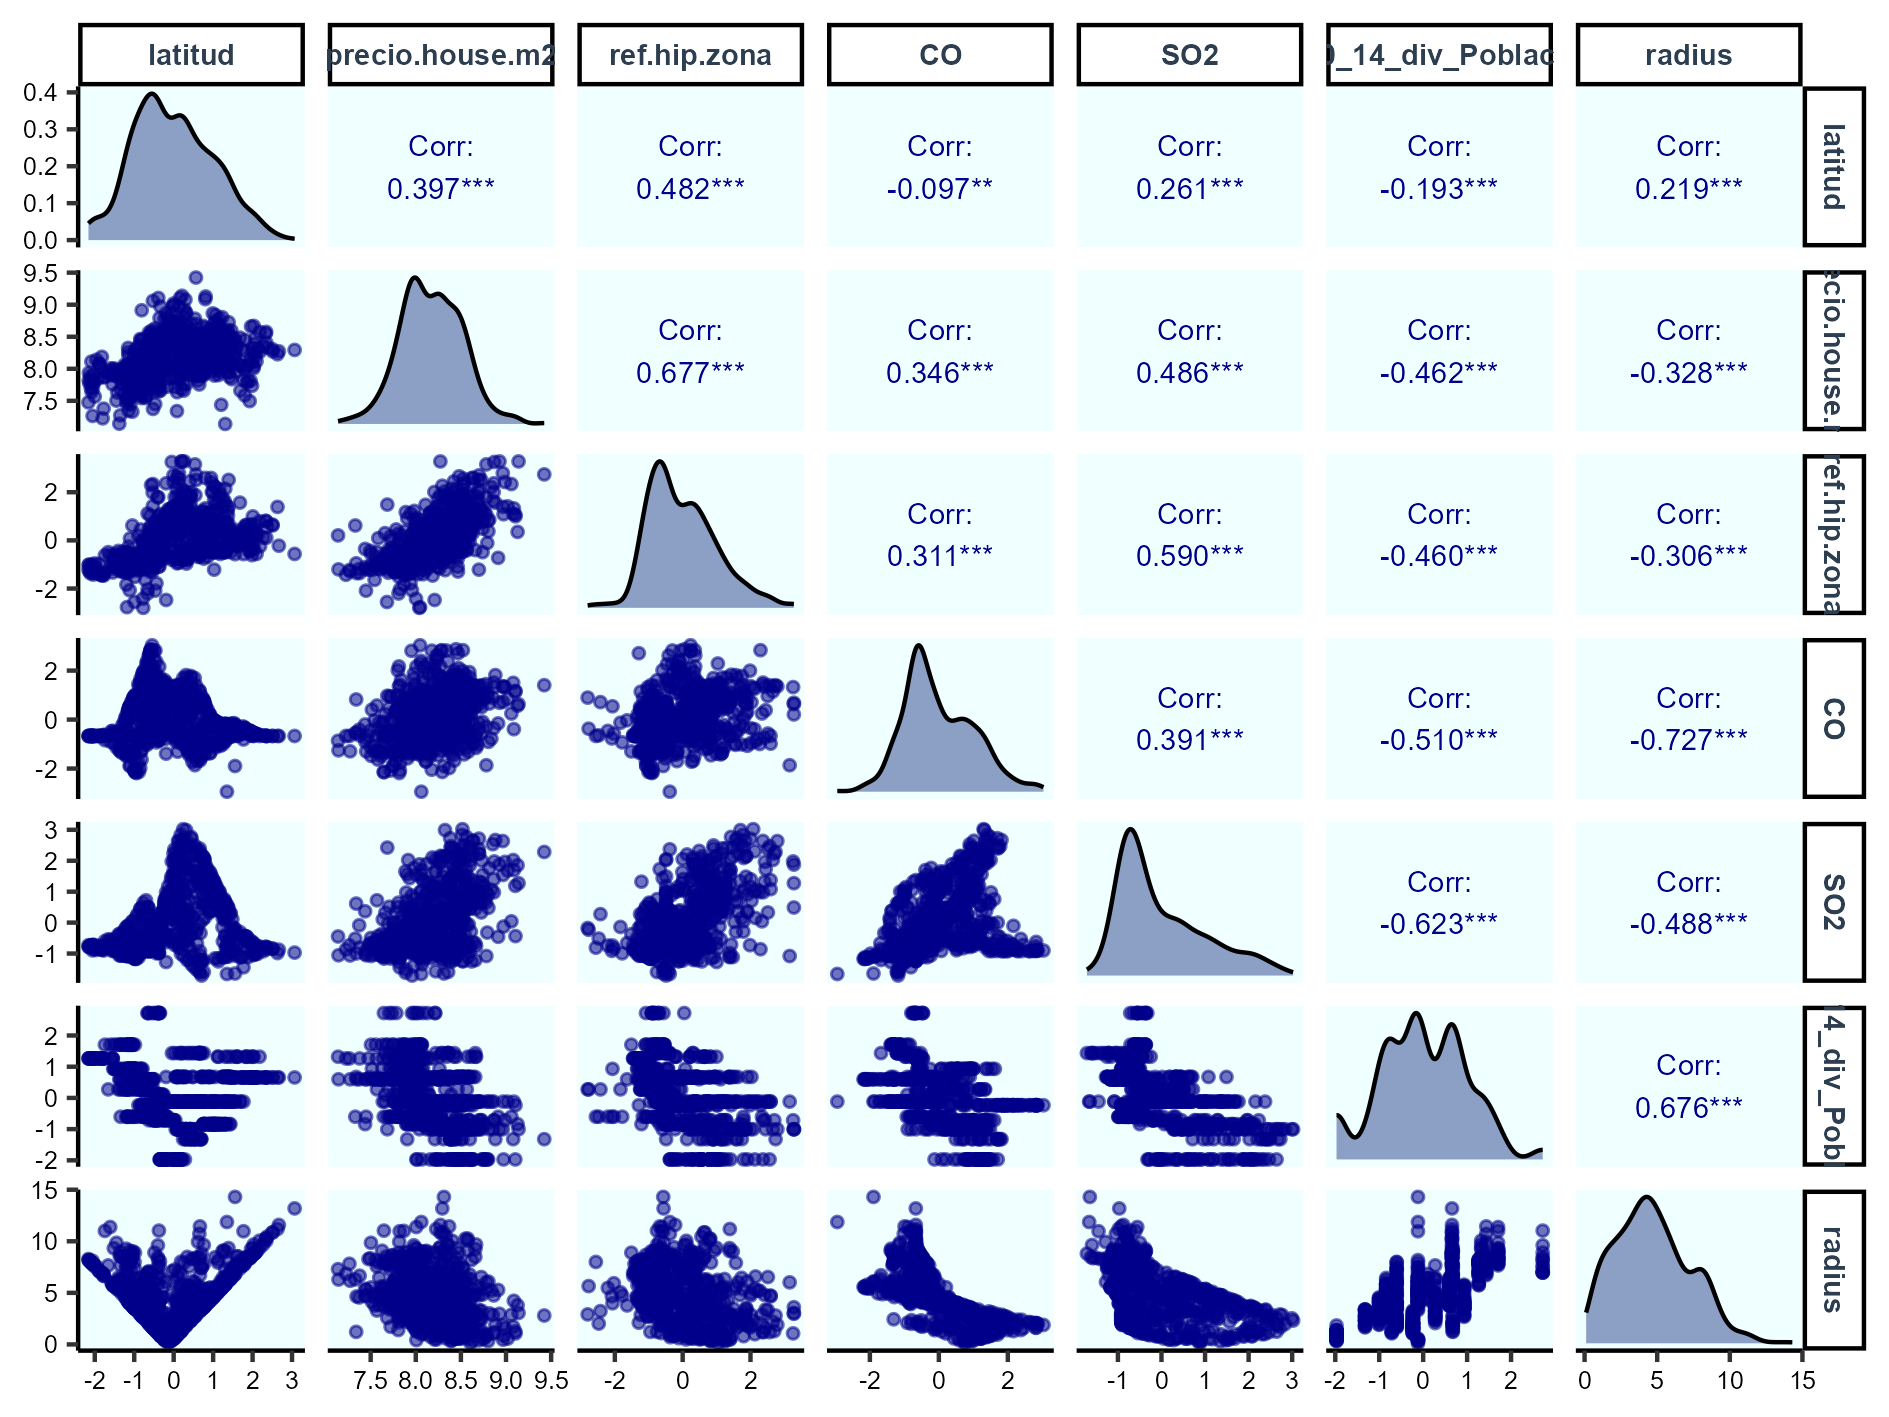
\includegraphics[width=0.8\textwidth]{Images/scatterplot_matrix.png} % 
    \caption{Scatterplot matrix of the most price-correlated variables}
    \label{fig:scatterplot_matrix} 
\end{figure}









\chapter{Prepossessing}\label{chap:preprocessing}

After studying the superficial distribution of the variables of the dataset the following modification will be implemented in order to improve the overall interpretability and performance of the regression models.

\section{Continuous Variables: Transformation of variables}

First of all, the predictor numerical variables in the dataset will be standardized to ensure that differences in scale and variability do not disproportionately influence the regression model coefficients. Standardization transforms variables so they have a mean value of zero and a standard deviation of one, allowing them to contribute equally to the model. Additionally this step is needed to perform some techniques like Ridge regression.

The distribution of the objective variables \textit{precio.house.m2} reveals a noticeable right skewness, deviating from normality. This deviation may impact some of the regression model assumptions, such as normality and homoscedasticity. To address this, the \textbf{logarithmic transformation} of the variable will be applied as a corrective measure.

\begin{figure}[h!]
    \centering
    % First subfigure
    \begin{subfigure}[b]{0.45\textwidth}
        \centering
        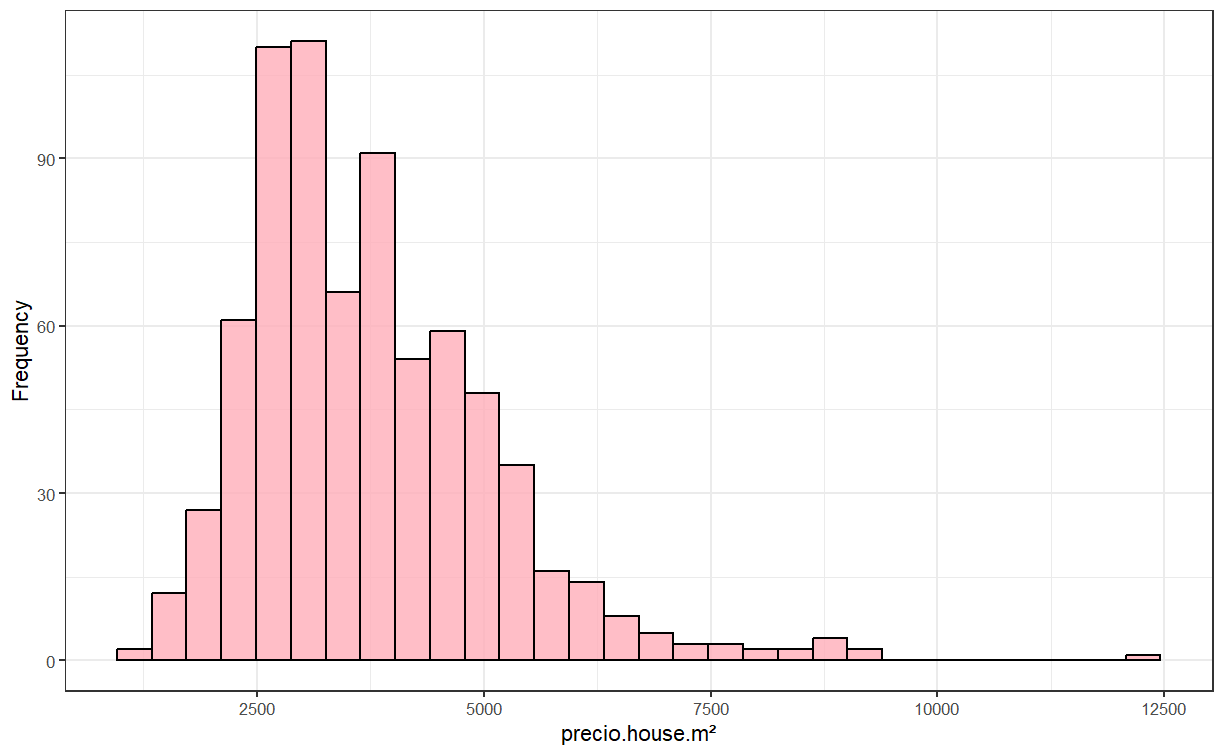
\includegraphics[width=\textwidth]{Images/Hist_price.png}
    \end{subfigure}
    \hfill
    % Second subfigure
    \begin{subfigure}[b]{0.45\textwidth}
        \centering
        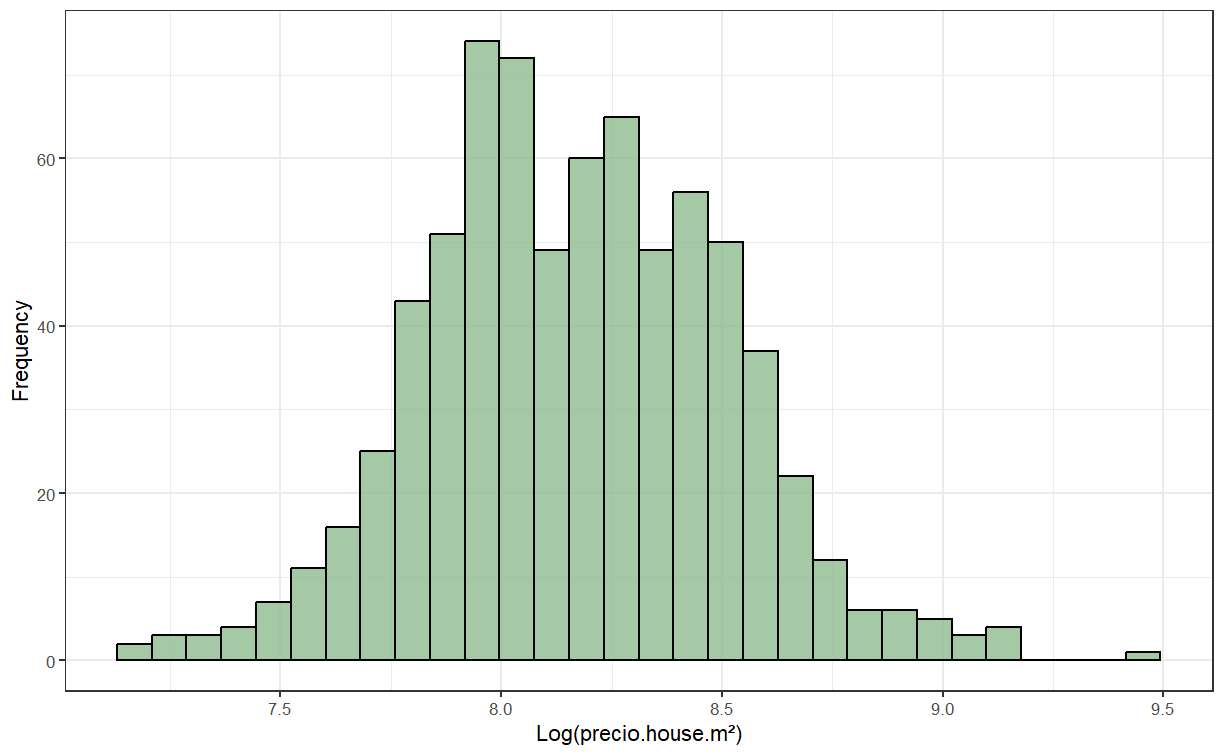
\includegraphics[width=\textwidth]{Images/Hist_log_price.png}
    \end{subfigure}
    \caption{Histogram of \textit{precio.house.m2} before and after logarithmic transformation}
    \label{fig:Hist_log_price}
\end{figure}


 
\section{Categorical Variables: Recategorization}

The dataset contains some categorical variables with an excessive number of levels. This makes model interpretability too complex. Moreover, a high number of categories can result in insufficient data for meaningful interactions with continuous variables, hence reducing the significance of the results. To address these issues, a recategorization of the variables has been implemented grouping those levels that present some rational similarities, ensuring that the number of categories remains reasonable. 

\begin{table}[H]
    \centering
    \begin{minipage}{0.35\textwidth}
        \centering
        \begin{tabular}{cccccccc}
            \toprule
            \textbf{dorm} & \textbf{0} & \textbf{1} & \textbf{2} & \textbf{3} & \textbf{4} & \textbf{5} & \textbf{6} \\ 
            \midrule
            \textbf{Count}       & 9      & 130    & 226    & 254    & 74     & 25     & 11     \\
            \textbf{\%}  & 1.04 & 15.06 & 26.14 & 29.39 & 8.56 & 2.89 & 1.27  \\ 
            \bottomrule
        \end{tabular}
    \end{minipage}
    \hfill
    \begin{minipage}{0.35\textwidth}
        \centering
        \begin{tabular}{ccccc}
            \toprule
            \textbf{dorm} & \textbf{0-1} & \textbf{2} & \textbf{3} & \textbf{$\geq$4} \\ 
            \midrule
            \textbf{Count}       & 139    & 226    & 254    & 117     \\ 
            \textbf{\%}  & 16.11 & 26.14 & 29.39 & 13.56 \\ 
            \bottomrule
        \end{tabular}
    \end{minipage}
    \caption{Comparison of the original and recategorized \textbf{room} distributions.}
    \label{tab:side_by_side_room_distribution}
\end{table}

\begin{table}[H]
    \centering
    \begin{minipage}{0.45\textwidth}
        \centering
        \begin{tabular}{cccccccc}
            \toprule
            \textbf{banos} & \textbf{1} & \textbf{2} & \textbf{3} & \textbf{4} & \textbf{5} & \textbf{6} & \textbf{7} \\ 
            \midrule
            \textbf{Count}       & 459    & 215    & 39     & 14     & 5      & 0      & 4      \\
            \textbf{\%}  & 62.36  & 29.21  & 5.29   & 1.90   & 0.67   & 0.00   & 0.54   \\ 
            \bottomrule
        \end{tabular}
    \end{minipage}
    \hfill
    \begin{minipage}{0.45\textwidth}
        \centering
        \begin{tabular}{cccc}
            \toprule
            \textbf{banos} & \textbf{1} & \textbf{2} & \textbf{$\geq$3} \\ 
            \midrule
            \textbf{Count}       & 459    & 215    & 62      \\ 
            \textbf{\%}  & 62.36  & 29.21  & 8.42    \\ 
            \bottomrule
        \end{tabular}
    \end{minipage}
    \caption{Comparison of the original and recategorized \textbf{bathroom} distributions.}
    \label{tab:side_by_side_distribution}
\end{table}

\begin{table}[H]
    \centering
    \resizebox{\textwidth}{!}{ % Scale the tables to fit the text width
        \begin{minipage}{0.575\textwidth}
            \centering
            \begin{tabular}{ccccccc}
                \toprule
                \textbf{tipo.casa} & \textbf{ático} & \textbf{chalet} & \textbf{dúplex} & \textbf{studio} & \textbf{otro} & \textbf{piso} \\ 
                \midrule
                \textbf{Count}       & 42    & 19    & 17     & 20     & 1      & 637     \\
                \textbf{\%}          & 5.71  & 2.58  & 2.31   & 2.71   & 0.14   & 96.55   \\ 
                \bottomrule
            \end{tabular}
        \end{minipage}
        \hfill
        \begin{minipage}{0.575\textwidth}
            \centering
            \begin{tabular}{ccccc}
                \toprule
                \textbf{tipo.casa} & \textbf{Chalet} & \textbf{Dúplex} & \textbf{Piso} & \textbf{Ático/Studio} \\ 
                \midrule
                \textbf{Count}       & 19     & 17     & 637     & 63      \\ 
                \textbf{\%}          & 2.58   & 2.31   & 96.55   & 9.56    \\ 
                \bottomrule
            \end{tabular}
        \end{minipage}
    }
    \caption{Comparison of the original and recategorized \textbf{type of property} distributions.}
    \label{tab:side_by_side_tipo_casa_distribution}
\end{table}


\begin{table}[H]
    \centering
    \resizebox{\textwidth}{!}{ % Scale to fit the page

        \begin{minipage}{0.695\textwidth}
            \centering
            \begin{tabular}{lccccccc}
                \toprule
                \textbf{estado} & \textbf{a-reformar} & \textbf{bueno} & \textbf{excelente} & \textbf{nuevo} & \textbf{reformado} & \textbf{malo} & \textbf{segunda-mano} \\ 
                \midrule
                \textbf{Count}       & 94    & 559   & 5     & 20     & 32      & 2      & 24     \\
                \textbf{\%}          & 12.77 & 75.95 & 0.68  & 2.72   & 4.35    & 0.27   & 3.26   \\ 
                \bottomrule
            \end{tabular}
        \end{minipage}
        \hfill
        \begin{minipage}{0.685\textwidth}
            \centering
            \begin{tabular}{lccc}
                \toprule
                \textbf{estado} & \textbf{Malo} & \textbf{Medio} & \textbf{Alto} \\ 
                \midrule
                \textbf{Count}       & 96     & 583     & 57      \\ 
                \textbf{\%}          & 13.74  & 79.21   & 7.74    \\ 
                \bottomrule
            \end{tabular}
        \end{minipage}
    }
    \caption{Comparison of the original and recategorized \textbf{state of the property} distributions.}
    \label{tab:side_by_side_estado_distribution}
\end{table}

The final categorical variable to be recategorized is \textit{distrito}. The districts will be grouped into broader geographical zones, this approach aligns with the observed distribution of property prices, providing a meaningful and interpretable grouping.

% \begin{itemize}
%     \item \textbf{South Districts:} Includes \textit{Carabanchel, Puente de Vallecas, Usera, Vallecas, Villaverde}

%     \item \textbf{Central Districts:} Includes \textit{Arganzuela, Centro, Chamberí, Retiro, Salamanca}

%     \item \textbf{North Districts:} Includes \textit{Barajas, Chamartín, Fuencarral, Hortaleza, Tetuán}

%     \item \textbf{West Districts:} Includes \textit{Moncloa, Latina}

%     \item \textbf{East Districts:} Includes \textit{Vallecas, Moratalaz, Vicálvaro, San Blas, Ciudad Lineal}
% \end{itemize}


% \begin{figure}
%     \centering
%     \includegraphics[width=1\linewidth]{Images/dist_final.png}
%     \caption{Grouping of districts}
%     \label{fig:district_grouping}
% \end{figure}

\section{Generation of Syntetic Variables}

\textbf{Radius}

To simplify the spatial information about each property that the dataset contains in the form of latitude and longitude while retaining as much relevant information as possible, the variable \textit{\textbf{radius}} has been created to represent the distance (in kilometers) between each property and the geographic center of Madrid, defined as Puerta del Sol. 
Appart from reducing dimensionality this approach provides also a direct and easily interpretable metric from the distance to the city center which often plays a significant role in real estate price.

\chapter{Modeling}\label{chap:modelling}

In order to test the models efficiency and ensure that they are not overfitting to the training data a k-fold cross-validation procedure will be implemented.

The dataset will be divided into four subsets, with each subset serving as the testing set once during the iterative process. In each iteration, the model will be trained on the remaining three folds. The chosen error metric will be calculated for each iteration, and the average of these values will be used to evaluate the overall performance of the model.

To ensure that the folds are properly balanced (meaning they contain a similar proportion of instances for each level of the categorical variables) a fixed seed has been set in the model code. This guarantees reproducibility and consistency in the cross-validation process. 

The choice of this seed was determined through the following process: a loop was implemented to test various seeds, calculating the proportions of each categorical variable across the folds, until optimal balance was achieved. As a result, the seed selected was \textbf{416}.

\begin{table}[h!]
    \centering
    \begin{tabular}{lcccc}
        \toprule
        \textbf{\%} & \textbf{C} & \textbf{NE} & \textbf{SE} & \textbf{SW} \\ 
        \midrule
        \textbf{Original} & 25.4 & 30.2 & 22.8 & 21.6 \\ 
        \textbf{k = 1} & 26.1 & 29.8 & 23.5 & 20.6 \\ 
        \textbf{k = 2} & 24.9 & 31.0 & 22.2 & 21.9 \\ 
        \textbf{k = 3} & 25.7 & 29.5 & 23.0 & 21.8 \\ 
        \textbf{k = 4} & 26.0 & 30.0 & 22.6 & 21.4 \\ 
        \bottomrule
    \end{tabular}
    \caption{Proportions of regions in different folds compared to the original dataset.}
    \label{tab:folds_comparison}
\end{table}



\chapter{Scoring}

\chapter{Results \& Conclusions}

\end{document}


